\documentclass{article}
\usepackage[utf8]{inputenc}
\usepackage{graphicx}
\graphicspath{ {./Images/} }
\setlength{\parskip}{0em}

\title{Cosmic Structure Formation}
\author{Samuel Hayes}
\date{\today}

\begin{document}

% Front Page
\maketitle
\vspace{40mm} %5mm vertical space
\begin{center}
    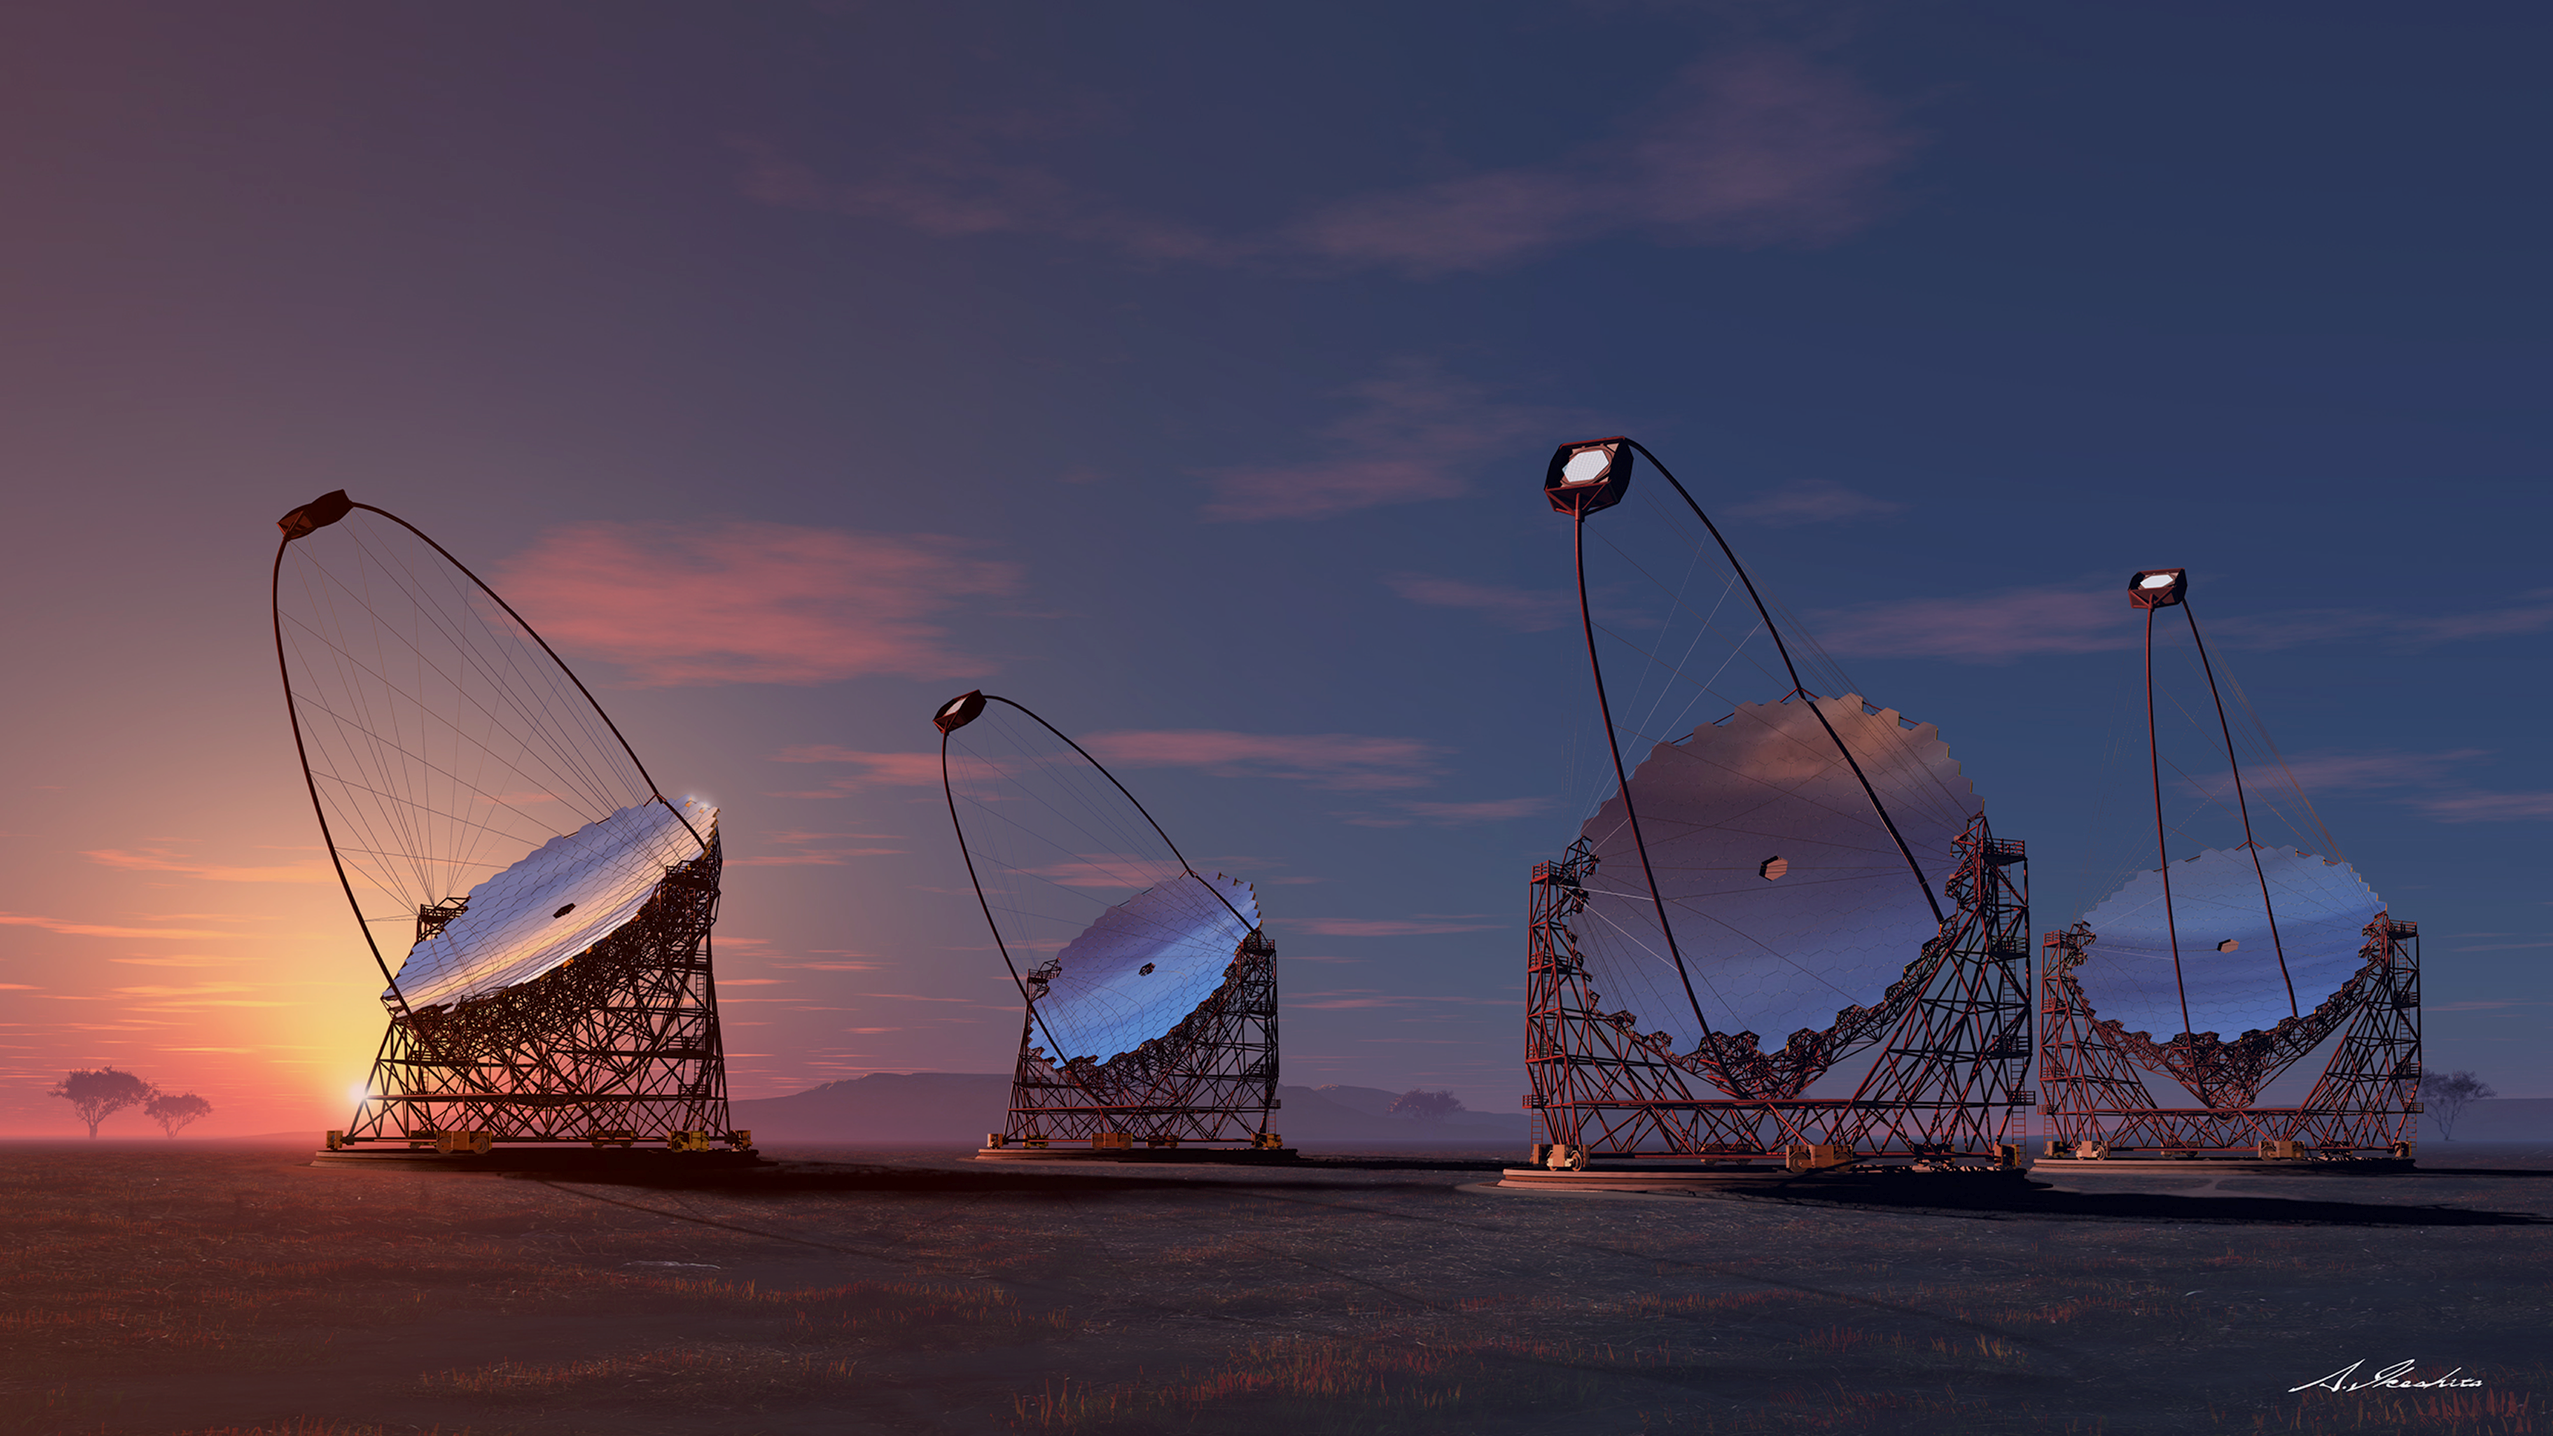
\includegraphics[width=\textwidth]{cherenkovTelescopeArray}
\end{center}

\newpage

% Table Of Contents
\tableofcontents
\newpage

% Main Goal of this Course
\section{Background Knowledge and Basics}

\subsection{Contents of the Universe}
The universe is comprised of many different elements all of which are balanced to produce the universe we know and love. For our universe these elements are balanced such that the total universe density is very close to the critical density causing the universe to be flat. Specifically they are:

\begin{itemize}
    \item $\Omega_\gamma = 5.1\times10^{-5}$ (Energy Density from Photons)
    \item $\Omega_{\nu , massless} = 3.4 \times 10^{-5}$ (Energy Density from massless neutrinos)
    \item $\Omega_{\nu , massive} = 0.06$ (Energy Density from massive neutrinos)
    \item $\Omega_{b} = 0.046$ (of which is stellar $\Omega_{*} = 0.0023$ (Energy Density from Baryons)
    \item $\Omega_{dm} = 0.23$ (Energy Density from Dark Matter)
    \item $\Omega_{\Lambda} = 0.73$ (Energy Density from Dark Energy / Vacuum Energy)
    
\end{itemize}

This uses the Density Parameter which is defined as:

\begin{equation}
    \Omega = \frac{\rho}{\rho_{crit}}
\end{equation}
\begin{equation}
    \rho_{crit} = \frac{3H(t)^2}{8\pi G}
\end{equation}

where $\rho$ is the density, $\rho_{crit}$ is the critical density, H(t) is the Hubble parameter at time t. This shows that we are living is a flat universe as by summing the main contributers to the density parameter we find that 
\begin{equation}
    \Omega = \Omega_{b} + \Omega_{dm} + \Omega_\Lambda \approx 1
\end{equation}
which corresponds to a flat universe, $k=0$.

\subsubsection*{Dark Matter}
Dark Matter is a construct that we know must exist due to the observational evidence of a source of mass which cannot be explained by any traditional baryonic source. It originated from observations of the rotation curves of galaxies, where virial velocities at higher velocities are higher than can be supported through the observed baryonic matter component (if there was only baryonic matter this high velocity section would not be gravitationally bound to the galaxy). This can be seen in (figure )

\begin{figure}
    \centering
    \includegraphics{}
    \caption{Caption}
    \label{fig:galaxyRotationCurve
\end{figure}

\end{document}
